\documentclass[11pt]{article}
\usepackage[utf8]{inputenc}
\usepackage[T1]{fontenc}
\usepackage{lmodern}
\usepackage{geometry}
\usepackage{tikz}
\usetikzlibrary{arrows.meta,shapes.geometric}

\geometry{paperwidth=13cm,paperheight=6.5cm,margin=0cm}
\pagestyle{empty}
\setlength{\parindent}{0pt}

\definecolor{ctxFill}{RGB}{238,242,245}
\definecolor{ctxLine}{RGB}{155,168,179}
\definecolor{ctxText}{RGB}{38,52,67}
\definecolor{exFill}{RGB}{220,233,247}
\definecolor{exLine}{RGB}{23,54,93}
\definecolor{prFill}{RGB}{200,240,236}
\definecolor{prLine}{RGB}{8,127,140}
\definecolor{prText}{RGB}{6,79,87}
\definecolor{phFill}{RGB}{234,242,245}

\begin{document}
\noindent
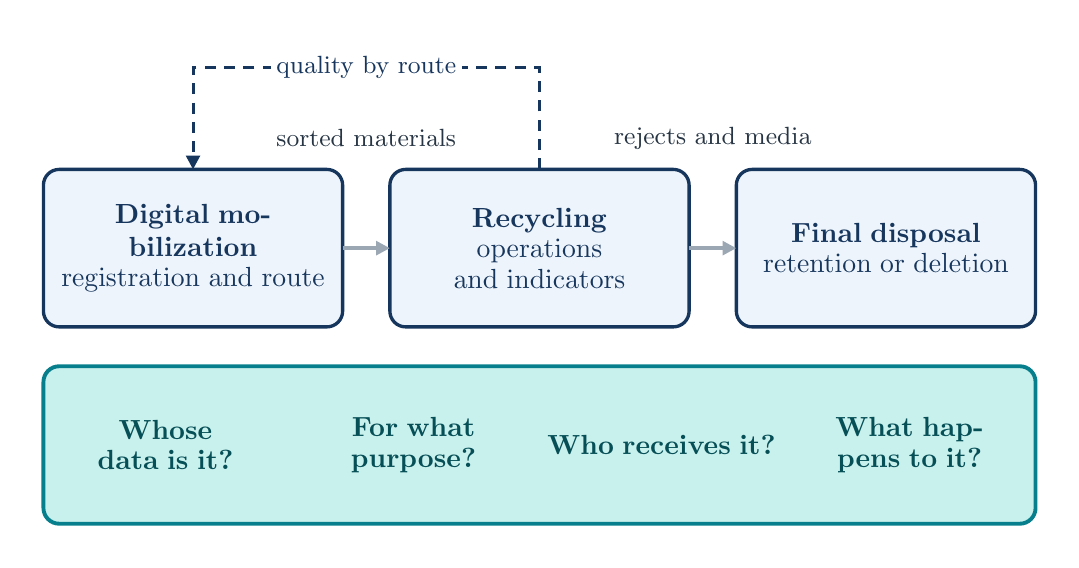
\begin{tikzpicture}[x=1cm,y=1cm,font=\small]
  \path[use as bounding box] (0,0) rectangle (13,6.5);
  \draw[fill=exFill!50,draw=exLine,line width=1.2pt,rounded corners=0.2cm] (0.2,2.7) rectangle (4.0,4.7);
  \node[align=center,text=exLine,text width=3.4cm] at (2.1,3.7) {\normalsize\textbf{Digital mobilization}\\ registration and route};
  \draw[fill=exFill!50,draw=exLine,line width=1.2pt,rounded corners=0.2cm] (4.6,2.7) rectangle (8.399999999999999,4.7);
  \node[align=center,text=exLine,text width=3.4cm] at (6.5,3.7) {\normalsize\textbf{Recycling}\\ operations and indicators};
  \draw[fill=exFill!50,draw=exLine,line width=1.2pt,rounded corners=0.2cm] (9.0,2.7) rectangle (12.8,4.7);
  \node[align=center,text=exLine,text width=3.4cm] at (10.9,3.7) {\normalsize\textbf{Final disposal}\\ retention or deletion};
  \draw[draw=ctxLine,line width=1.2pt,-{Triangle[length=5pt,width=5pt]}] (4.0,3.7) -- (4.6,3.7);
  \draw[draw=ctxLine,line width=1.2pt,-{Triangle[length=5pt,width=5pt]}] (8.4,3.7) -- (9.0,3.7);
  \node[text=ctxText,align=center] at (4.3,5.1) {\small sorted materials};
  \node[text=ctxText,align=center] at (8.7,5.1) {\small rejects and media};
  \draw[draw=exLine,line width=1.1pt,dash pattern=on 4pt off 3pt,-{Triangle[length=5pt,width=5pt]}] (6.5,4.7) -- (6.5,6.0) -- (2.1,6.0) -- (2.1,4.7);
  \node[text=exLine,fill=white,inner sep=2pt] at (4.3,6.0) {\small quality by route};
  \draw[fill=prFill,draw=prLine,line width=1.4pt,rounded corners=0.2cm] (0.2,0.2) rectangle (12.8,2.2);
  \node[text=prText,align=center,text width=2.9cm] at (1.75,1.2) {\normalsize\textbf{Whose data is it?}};
  \node[text=prText,align=center,text width=2.9cm] at (4.9,1.2) {\normalsize\textbf{For what purpose?}};
  \node[text=prText,align=center,text width=2.9cm] at (8.05,1.2) {\normalsize\textbf{Who receives it?}};
  \node[text=prText,align=center,text width=2.9cm] at (11.2,1.2) {\normalsize\textbf{What happens to it?}};
\end{tikzpicture}
\end{document}
